\atstartofhistorysection
\section[Un peu d’histoire : le moteur compound]{Un peu d’histoire :\onlyamphibook{\\} le moteur compound}

%	\textit{ou : la série de pistons transatlantique}
	Dans les années 1830, le moteur à vapeur vient de révolutionner le paysage et le réseau économique de la Grande-Bretagne. Tout y voyage alors par rail : passagers, récoltes, charbon, produits de l’industrie. Tout cela est tracté par des moteurs à vapeur, aux dimensions monumentales et à l’efficacité déplorable (on parle alors de trois pourcent). Ce n’est pas dramatique : le charbon et l’eau abondent, et il suffit d’arrêts ponctuels le long des lignes de chemin de fer pour réapprovisionner les machines.

	Sur les océans, la situation n’est pas la même : c’est encore la voile qui mène le jeu. Pour pouvoir joindre deux continents au moteur (c’est à dire sans louvoyer !), il faut résoudre deux problèmes.

	Le premier est que les moteurs consomment beaucoup d’eau. L’eau de mer, certes abondante, est inutilisable en l’état car les dépôts de sel et de calcaire provoqués lors de son ébullition étouffent les chaudières et entraînent un grave risque d’explosion. Il faut donc la désaliniser si l’on veut l’insérer dans la chaudière, ce qui est très coûteux en énergie.

	Le problème sera résolu avec l’utilisation des \textit{condenseurs}, dont les locomotives étaient dispensées par économie de place. Désormais, lorsque la vapeur a effectué son travail dans les cylindres, elle n’est plus simplement jetée dans l’atmosphère, mais refroidie dans de grands condenseurs avant d’être comprimée puis ré-insérée dans la chaudière. L’eau circule donc de façon cyclique à travers tout le moteur --\ il n’est plus besoin que de pallier les fuites.

	Le second problème est plus grave et plus difficile à résoudre : comment augmenter le rendement ? Ce n’est pas qu’une question financière : le premier navire transatlantique à vapeur, le \textit{SS Savannah}, termine sa traversée à la voile, alors qu’il n’était empli \emph{que} du charbon de son moteur !

	\begin{figure}
		\begin{center}
			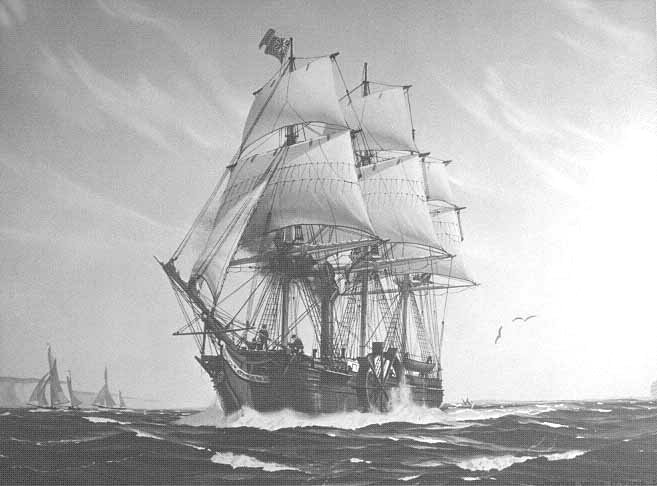
\includegraphics[width=0.7\textwidth]{images/ss_savannah.jpg}
		\end{center}
		\supercaption{\textit{SS Savannah}, première traversée atlantique à vapeur en 1819, terminée à la voile.}{Image \pd \wcfile{SS-Savannah.jpg}{par Hunter Wood, 1819}}
		\onlyamphibook{\vspace{-2.5em}}
	\end{figure}

	Pour augmenter le rendement d’un moteur de capacité donnée, on cherche à augmenter la quantité de travail générée par chaque kilo de vapeur, qui peut être approximée par la relation~\ref{eq_travail_pdv} :

	\begin{equation*}
	w_\fromatob = - \int _{\A}^\B {p \diff v}
	\end{equation*}

	La première chose à faire est d’augmenter la pression $p_A$ de la vapeur, c’est à dire sa pression avant qu’elle ne débute sa détente dans les cylindres. Ce n’est pas chose facile : augmenter la pression de la chaudière augmente les contraintes structurelles qu’elle subit, donc son coût, et réduit son efficacité car les parois doivent être épaissies et alourdies.

	On peut ensuite tenter d’augmenter le $\Delta v $, c’est-à-dire la variation totale de volume lors du mouvement du piston. Autrement dit, il faut augmenter le volume balayé par les cylindres. Là encore, ce n’est pas chose facile.
	
	D’une part, lorsque l’on augmente le diamètre des cylindres --\ ce qui augmente l’aire~$S$\ -- on soumet les pistons à une plus grande force $F_A$, pour une pression $p_A$ donnée (\ref{def_pression}) :
	\begin{equation*}
	p \equiv \frac{F}{S}
	\end{equation*}
	En augmentant la force transmise, on atteint rapidement les limites structurelles de la mécanique motrice.

	D’autre part, lorsque l’on augmente la longueur des cylindres, on rallonge également le moteur et on alourdit considérablement le mécanisme de bielle/ et vile\-brequin. D’autant que la pression et le volume de la vapeur sont liés l’un à l’autre : ils suivent approximativement une relation de type $p v^{x} = k$ pendant la détente. Autrement dit, plus le volume augmente, plus la pression diminue : au fur et à mesure que l’on rallonge le cylindre, les gains en travail sont de plus en plus faibles.

	Le moteur \vocab{compound} répond à ce problème en utilisant plusieurs cylindres \textit{en série} (\cref{fig_cylindres_compound}). La vapeur à haute pression déplace d’abord un piston de petit diamètre (limitant ainsi la force exercée sur le mécanisme). Ensuite, elle est transférée dans un autre cylindre, de plus grand diamètre. Celui-ci permet d’obtenir une force identique avec une pression plus basse ; il balaie un plus grand volume.

	\begin{figure}
		\begin{center}
			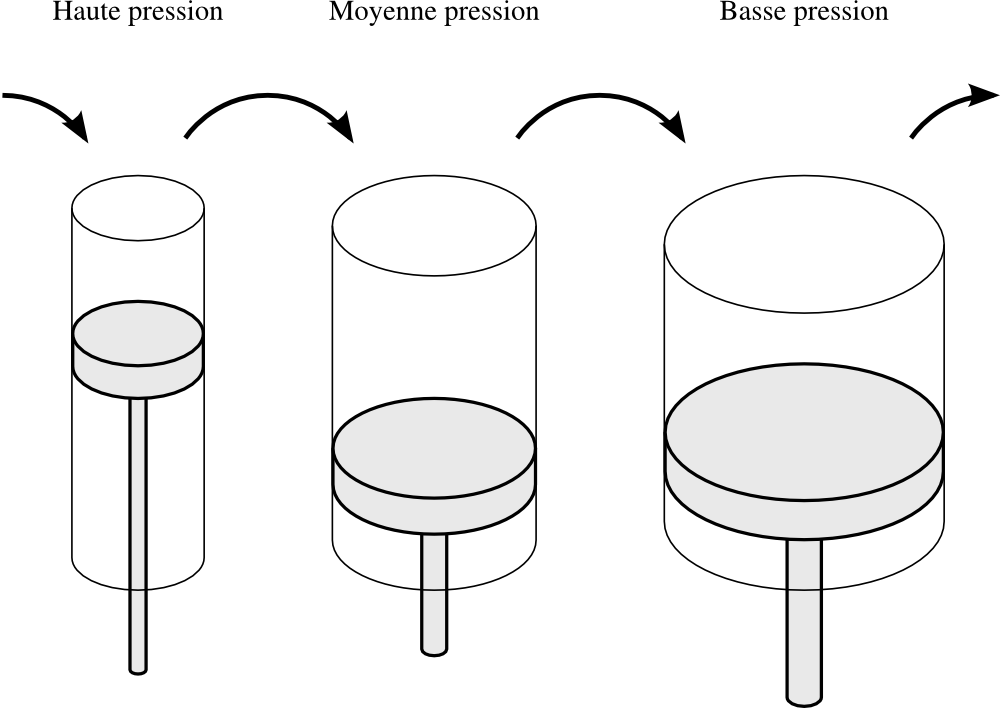
\includegraphics[width=0.8\textwidth]{images/cylindres_compound.png}
			\onlyamphibook{\vspace{-1cm}}
		\end{center}
		\supercaption{Cylindres en série, dits \textit{compound}.}{schéma \ccbysa \olivier}
		\label{fig_cylindres_compound}
			\onlyamphibook{\vspace{-1em}}
	\end{figure}

	Ainsi, en augmentant le volume total balayé par la vapeur en expansion, on peut extraire plus de travail de la vapeur compressée, sans surdimensionner le vilebrequin ni surcharger les pistons.

	Avec un tel moteur, la marine marchande est capable d’abandonner le cabotage : elle s’empare de cette nouvelle technologie qui connaît un succès immédiat. De deux cylindres en série (\vocab{double compound}) on passe à trois, et même parfois quatre (\vocab{quadruple compound}!), pour extraire de la vapeur à chaque fois plus d’énergie, sous forme de travail.

	\begin{figure}
		\begin{center}
			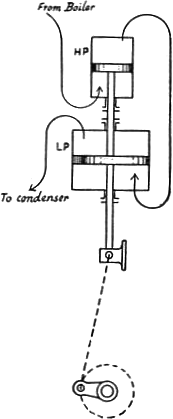
\includegraphics[height=11cm, max height=0.55\textheight]{images/ripper_compound_1.png}
			%\vspace{0.5cm}
			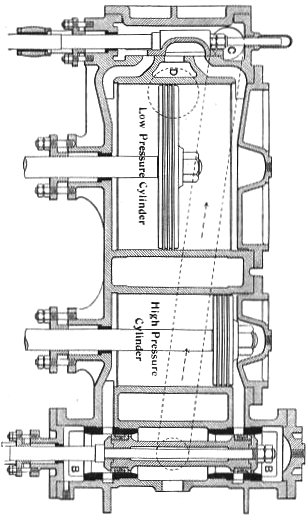
\includegraphics[height=10cm, max height=0.55\textheight]{images/ripper_compound_2.png}
		\end{center}
		\supercaption{Différents systèmes compound à vapeur.}{Images \pd \wcfile{Compound engine with both piston and slide valves (Heat Engines, 1913).png}{Prof. William Ripper, 1889}}
	\end{figure}

	L’enthousiasme gagne les armateurs, qui se targuent désormais ne plus devoir brûler qu’une feuille de papier pour déplacer une tonne de cargaison sur un mile. Même s’il s’entend que ledit papier est fort épais, l’avancée est faite. Voilà le thé des Indes bientôt dans les tasses londoniennes --\ l’empire britannique dispose à partir de ce moment des machines dont avait besoin son formidable réseau économique.
\atendofhistorysection
